\documentclass[11pt]{article}
\usepackage[margin=2cm]{geometry}
\usepackage{booktabs,makecell,graphicx,amsmath}
\begin{document}
\section*{Step 0 asset preview}
\begin{table}[h]\centering\footnotesize
\caption{Task completion and action interface (Exp.~1).}
\resizebox{\linewidth}{!}{\begin{tabular}{llcccccrr}
\toprule
Model & Interface & \makecell{Success\\(\%)} & \makecell{Exact optimal\\(\%)} & \makecell{Near-opt.\\(\%)} & \makecell{$\Delta J$ median / max\\(GBP)} & \makecell{Max $\gamma$\\(\%)} & Tokens & \makecell{\$ per\\success} \\
\midrule
GPT-4o-mini & FC & 100 [76,\,100] & 100 [76,\,100] & 100 & 0.00 / 0.00 & 0.0 & 7,364 & 0.0013 \\
 & Text & 94 [68,\,99] & 31 [12,\,58] & 39 & 0.14 / 0.83 & 12.7 & 38,712 & 0.0073 \\
Gemini 2.5 Flash & FC & 100 [76,\,100] & 100 [76,\,100] & 100 & 0.00 / 0.00 & 0.0 & 6,894 & 0.0048 \\
 & Text & 92 [65,\,99] & 64 [37,\,84] & 89 & 0.00 / 0.08 & 2.0 & 57,328 & 0.0522 \\
Claude Sonnet 4.6 & FC & 100 [76,\,100] & 86 [58,\,97] & 97 & 0.00 / 0.33 & 4.4 & 11,790 & 0.0489 \\
 & Text & 50 [25,\,75] & 33 [14,\,61] & 47 & 0.00 / 0.31 & 3.4 & 17,155 & 0.1843 \\
\midrule
Llama-3.3 70B & FC & 97 [72,\,100] & 36 [16,\,63] & 78 & 0.00 / 0.56 & 8.5 & 25,629 & 0.0035 \\
 & Text & 81 [52,\,94] & 31 [12,\,58] & 67 & 0.00 / 0.53 & 5.6 & 47,437 & 0.0091 \\
Qwen-3 32B & FC & 100 [76,\,100] & 72 [44,\,90] & 86 & 0.00 / 1.86 & 122.9 & 26,120 & 0.0027 \\
 & Text & 75 [47,\,91] & 47 [23,\,72] & 56 & 0.00 / 0.27 & 3.2 & 29,054 & 0.0043 \\
\bottomrule
\end{tabular}
}\end{table}
\begin{table}[h]\centering\footnotesize
\caption{Direct, guard and hybrid under constraint conflict (Exp.~2).}
\resizebox{\linewidth}{!}{\begin{tabular}{lcccccc}
\toprule
Model & \makecell{Direct\\(\%)} & \makecell{Guard\\(\%)} & \makecell{Hybrid\\(\%)} & \makecell{Hybrid $-$ direct\\(pp)} & \makecell{Invalid commits\\direct $\to$ hybrid} & \makecell{\$ per correct\\direct / hybrid} \\
\midrule
GPT-4o-mini & 72 [45,\,89] & 87 [61,\,97] & 82 [55,\,94] & +10 [-13,\,+33] & 9 $\to$ 0 & 0.0037 / 0.0008 \\
Gemini 2.5 Flash & 97 [73,\,100] & 97 [73,\,100] & 100 [77,\,100] & +3 [+0,\,+8] & 0 $\to$ 0 & 0.0151 / 0.0018 \\
Claude Sonnet 4.6 & 100 [77,\,100] & 100 [77,\,100] & 100 [77,\,100] & +0 [+0,\,+0] & 0 $\to$ 0 & 0.0846 / 0.0221 \\
\midrule
Llama-3.3 70B & 38 [18,\,64] & 59 [33,\,81] & 90 [64,\,98] & +51 [+31,\,+69] & 5 $\to$ 3 & 0.0097 / 0.0006 \\
Qwen-3 32B & 79 [52,\,93] & 64 [38,\,84] & 64 [38,\,84] & -15 [-41,\,+10] & 3 $\to$ 3 & 0.0040 / 0.0005 \\
\bottomrule
\end{tabular}
}\end{table}
\begin{table}[h]\centering\footnotesize
\caption{Sources of hybrid failures.}
\resizebox{\linewidth}{!}{\begin{tabular}{llrll}
\toprule
Type & Cause & Runs & Models & Scenarios \\
\midrule
Interpretation & Dropped or loosened the EV deadline $\Rightarrow$ invalid commit & 6 & Llama-3.3 3, Qwen-3 3 & S5 \\
 & Invented a power cap $\Rightarrow$ false infeasibility & 6 & Qwen-3 6 & S1a, S1d, S3c \\
 & Invented an EV earliest start $\Rightarrow$ false infeasibility & 5 & Llama-3.3 1, Qwen-3 4 & S3a, S3b \\
 & Invented a washing-machine deadline $\Rightarrow$ false infeasibility & 4 & GPT-4o-mini 4 & S2a, S2b \\
 & Invented several constraints $\Rightarrow$ false infeasibility & 1 & Qwen-3 1 & S3b \\
\midrule
Protocol & Did not retry after the injected tool failure & 2 & GPT-4o-mini 2 & S6 \\
 & No optimizer call and no infeasibility report & 1 & GPT-4o-mini 1 & S4b \\
\midrule
 & Total & 25 & \multicolumn{2}{l}{22 interpretation, 3 protocol} \\
\bottomrule
\end{tabular}
}\end{table}
\begin{table}[h]\centering\footnotesize
\caption{Realized net cost (GBP/day) by weather regime (Exp.~3).}
\resizebox{\linewidth}{!}{\begin{tabular}{lcccccccc}
\toprule
 & \multicolumn{3}{c}{LLM agents (matched model-days)} & \multicolumn{3}{c}{MILP references} & \\
\cmidrule(lr){2-4}\cmidrule(lr){5-7}
Regime & \makecell{Direct,\\price-only} & \makecell{Direct,\\weather tools} & Hybrid & \makecell{Price-\\only} & \makecell{Weather-\\aware} & \makecell{Perfect\\foresight} & \makecell{Hybrid captures\\(\%)} \\
\midrule
Overcast & 4.477 & 4.513 & 4.382 & 4.469 & 4.378 & 4.330 & 96 \\
Mixed & 5.441 & 5.436 & 5.332 & 5.427 & 5.332 & 5.305 & 100 \\
Sunny & 3.516 & 3.562 & 3.302 & 3.517 & 3.302 & 3.302 & 100 \\
\bottomrule
\end{tabular}
}\end{table}
\begin{table}[h]\centering\footnotesize
\caption{Seven-day deployment (Exp.~4a).}
\resizebox{\linewidth}{!}{\begin{tabular}{lcccc}
\toprule
Policy & \makecell{Seven-day cost\\(GBP)} & \makecell{EV deadline\\met (days)} & \makecell{Timer-to-oracle\\savings captured (\%)} & \makecell{Weather value\\captured (\%)} \\
\midrule
Immediate start & 72.13 & 0/7 & -76.8 & -- \\
Off-peak timer & 51.27 & 7/7 & 0.0 & -- \\
Greedy cheapest-slot heuristic & 55.33 & 0/7 & -14.9 & -- \\
\midrule
Price-only MILP & 24.62 & 7/7 & 98.1 & 0.0 \\
Weather-aware MILP (oracle) & 24.10 & 7/7 & 100.0 & 100.0 \\
Perfect-foresight MILP & 24.05 & 7/7 & 100.2 & 108.5 \\
\midrule
GPT-4o-mini agent & 24.63 & 7/7 & 98.0 & -2.2 \\
Gemini 2.5 Flash agent & 24.77 & 7/7 & 97.5 & -29.2 \\
Claude Sonnet 4.6 agent & 25.00 & 7/7 & 96.7 & -73.8 \\
\bottomrule
\end{tabular}
}\end{table}
\begin{table}[h]\centering\footnotesize
\caption{Appendix: direct agent, baseline/guided prompt, with severity.}
\resizebox{\linewidth}{!}{\begin{tabular}{lccccccccc}
\toprule
Model & S1 & S2 & S3 & S4 & S5 & S6 & \makecell{Invalid\\commits} & \makecell{Worst\\overrun (h)} & \makecell{Worst cap\\excess (kW)} \\
\midrule
GPT-4o-mini & 1.00/1.00 & 0.00/0.00 & 0.67/0.78 & 0.50/1.00 & 0.00/0.00 & 1.00/1.00 & 21/74 & 9.0 & 2.2 \\
Gemini 2.5 Flash & 0.92/1.00 & 1.00/1.00 & 1.00/1.00 & 1.00/0.83 & 0.33/1.00 & 0.67/1.00 & 1/70 & 8.5 & -- \\
Claude Sonnet 4.6 & 1.00/1.00 & 1.00/1.00 & 1.00/1.00 & 1.00/1.00 & 1.00/1.00 & 1.00/1.00 & 0/78 & -- & -- \\
\midrule
Llama-3.3 70B & 0.67/0.58 & 0.50/0.67 & 0.56/0.33 & 0.50/0.00 & 0.67/0.00 & 1.00/0.33 & 14/50 & 7.5 & 2.2 \\
Qwen-3 32B & 0.75/0.92 & 1.00/1.00 & 0.67/1.00 & 0.17/0.67 & 0.00/0.00 & 1.00/0.33 & 16/71 & 9.5 & -- \\
\bottomrule
\end{tabular}
}\end{table}
\clearpage
\begin{figure}[h]\centering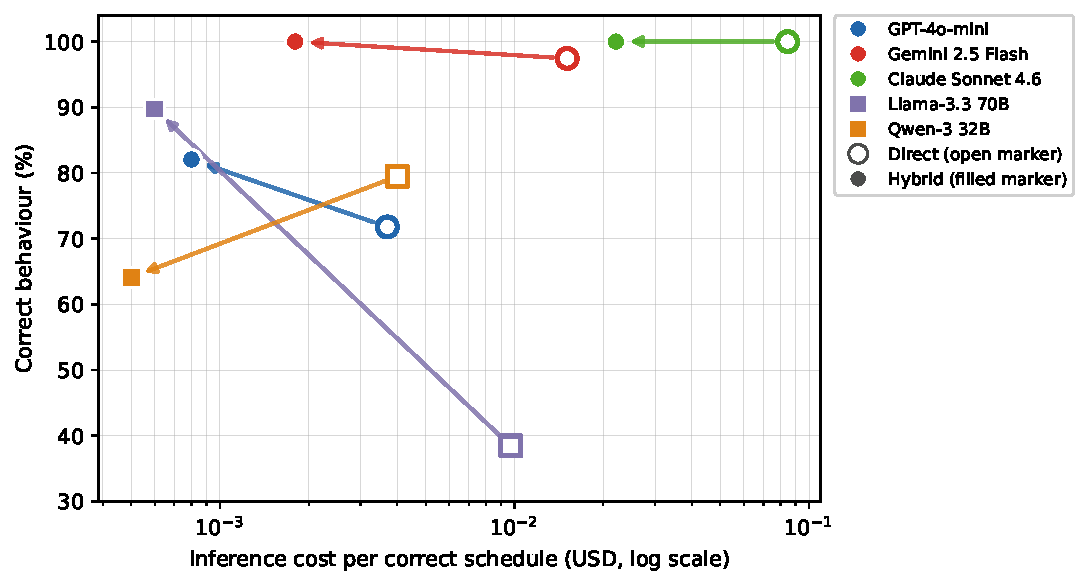
\includegraphics[width=0.75\linewidth]{fig_efficiency.pdf}
\caption{Correct behaviour vs cost per correct schedule, direct to hybrid.}\end{figure}
\begin{figure}[h]\centering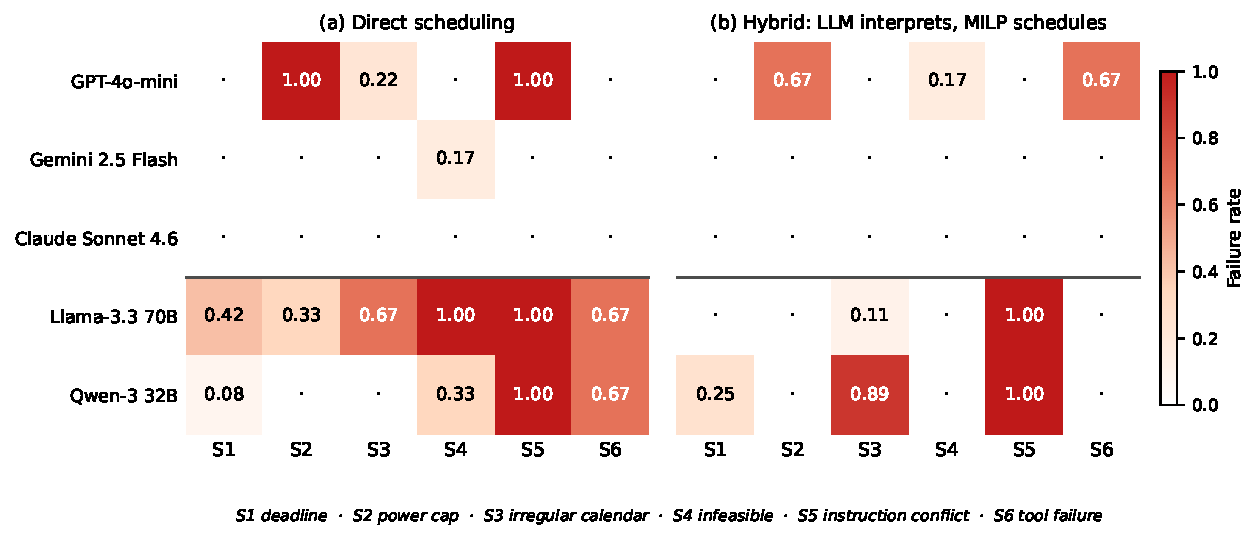
\includegraphics[width=\linewidth]{fig_direct_vs_hybrid.pdf}
\caption{Failure rate by scenario family, direct vs hybrid.}\end{figure}
\begin{figure}[h]\centering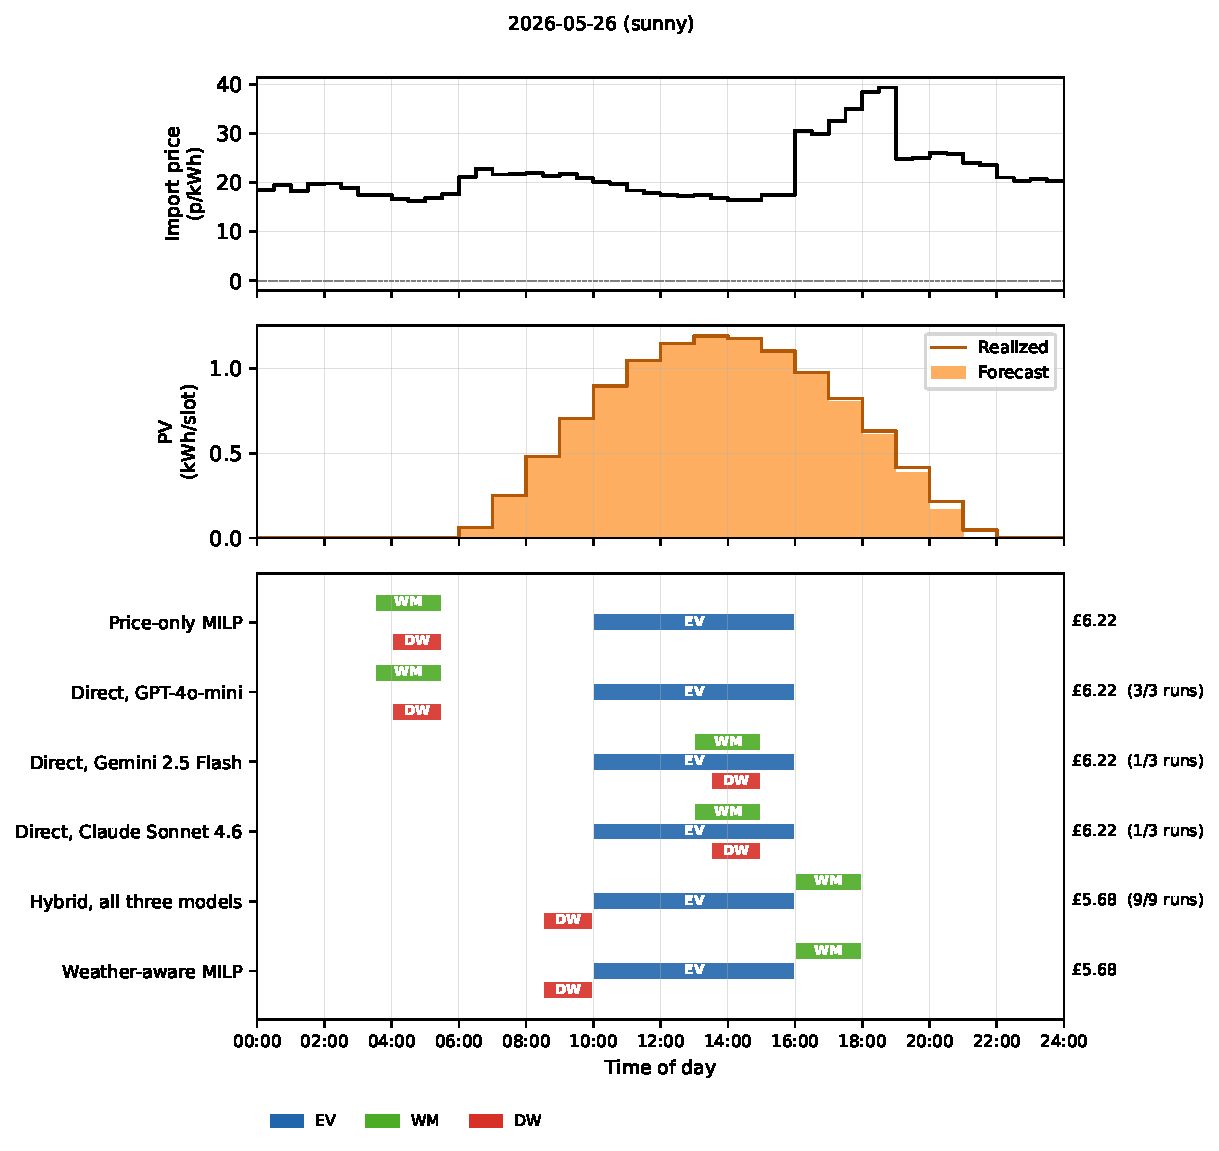
\includegraphics[width=0.9\linewidth]{fig_sunny_day.pdf}
\caption{Illustrative sunny day.}\end{figure}
\end{document}
